% ---------- SECTION IV - FIDO2 & WebAuthn ----------

\section{Results}
\label{sec:results}

To answer the research question, the literature is analyzed for two main topics: usability and security.\\
While there is some amount of research regarding the usability of \ac{fido2}, literature regarding the preceding protocols \ac{u2f} and \ac{uaf} is also taken into account due to the similarity of the involved hardware and authentication flows.\\
The security part of this chapter is mainly based on evaluations of the proposed concepts and mechanisms, as there is not yet any research regarding the security of actual implementations of either hardware or protocols.

% ---- Subsection Usability ----
\subsection{Usability}
\label{subsec:usability}

To determine whether a new authentication concept is accepted by users, and could therefore replace passwords, the usability plays a significant role. Regular passwords have been the prevalent authentication mechanism since the 1960's \cite{mcmillan2012}, so people are very familiar with their usage. The concept of sending credentials, checking them, and granting access to the protected ressource is also very intuitive. Using a hardware token, or in case of internal authenticators only a system dialogue, is a radically different approach.\\
A good starting point to evaluate whether this hardware-dependent approach is suitable is the study conducted by Lang et al \cite{lang2017}. The authors analyzed the roll-out of hardware tokens for 50,000 employees of Google as a second factor. In comparison to other \ac{2fa} methods like \ac{totp}, they found using a security key to be significantly faster.\\
On the other hand, a more qualitative and in-depth study of Das et al (2018) showed major usability problems for participants without technical backgrounds, especially during the initial setup. They report that users had trouble finding the correct instructions and where not able to intuitively use the device, as they had not yet developed a mental model regarding the functionality of the keys. The authors also explicitly state that one of the major problems was that users still had to enter their passwords, leading to additional work and complexity without any perceived benefit \cite{das2018}. This factor becomes less of a problem when a \ac{fido2} token is used for passwordless authentication.\\
\\
The most important scientific work for this section is a recent study by Lyastani et al, published in 2020, that focuses on the usability of \ac{fido2} as a means of passwordless, \ac{1fa}. They conclude that participants rated logging in via \ac{fido2} and an external authenticator as more usable than standard passwords, and were able to show a higher acceptance than the latter \cite{lyastani2020}.\\
However, the authors also identified some challenges, of which the most important ones are listed below:

\begin{description}
    \item[Complex Setup] Especially the initial registration of the key was seen as a challenge by many participants, this corresponds with the findings of \cite{das2018}.
    \item[Requires Physical Device] Users criticized that they had to carry an authenticator, and that the absence of this devices effectively logs them out of the application, substantially limiting spontaneous use.
    \item[Support of Other Devices] Logging in on devices without any way to connect the authenticator (e.g. a tablet or public PC without USB-A ports or NFC) is impossible.
    \item[Account Recovery after Loss] If the security key gets lost or stolen, account recovery is much more complex than with passwords. The current recommendation is to register a second backup key with each account \cite{gomi2019}.
    \item[No Account Delegation] It is not possible to grant a trusted third party (e.g. a colleague) access to an account without giving away the hardware key.
\end{description}

The above findings are now applied to the framework proposed by Nielsen (1993), where acceptability is split into social and practical acceptability. Due to the lack of literature and practical relevance, only the practical usability of \ac{fido2} is considered in this paper.\\
Practical acceptability is now divided into \emph{cost}, \emph{compatibility}, \emph{reliability} and \emph{usefulness} \cite[25 \psq]{nielsen1993}:

\begin{description}
    \item[Cost] In the study by \cite{lyastani2020}, around a third of the participants stated that they would rather not use \ac{fido2} due to the cost of external authenticators. This is partly countered by the possible use of internal authenticators (such as a Windows 10 PC or an Android Smartphone), but if a roaming authenticator is required for mobility, prices range between 20€ and 45€ per key \cite{yubikey_5_nfc} - which means at least 40€ if a backup key is registered.
    \item[Compatibility] As WebAuthn is a browser protocol that is currently implemented in almost every major browser, compatibility should not be an issue. Additionally, it is currently supported in Windows 10 and Android, with full support for Apples iOS on its way \cite{nichols2020}. As \ac{ctap} and WebAuthn are open standards, compatibility should increase in the near future.
    \item[Reliability] The reliability of a \ac{fido2} authentication is hard to estimate, as many components are required to work. For WebAuthn, the standardisation by the \ac{w3c} should be enough to conclude that it is robust. An unknown factor are hardware keys, as their reliability depends on the manufacturer.
\end{description}

The usability, according to \cite[25 \psq]{nielsen1993} a sub-component of \emph{usefulness}\footnote{The other sub-component, \emph{utility}, is not further evaluated in this paper.}, is again divided into five metrics, that are evaluated in the following paragraph:

\begin{description}
    \item[Easy to learn] The basic usage of the FIDO2 framework is easy to learn, although better and more user-friendly documentation is required as most people are only used to passwords \cite{lyastani2020,hunt2018b,das2018}.
    \item[Efficient to use] Using a security key is very fast once the users have learned it \cite{lang2017}.
    \item[Easy to remember] As the process of loggin in itself is quite simple and, contrary to passwords, identical for each application, it should be easy to reproduce. Nevertheless, there is currently no long-term research to further support this evaluation.
    \item[Few errors] Once setup correctly, there is very little room for errors. However, this also depends on the authenticator used, as for example biometrics could confuse a user and therefore introduce errors \cite{lyastani2020}.
    \item[Subjectively pleasing] Participants in recent studies have found security keys enjoyable to use in \ac{1fa} scenarios \citep{lyastani2020}, but were less convinced in \ac{2fa} settings \cite{das2018}.
\end{description}

There is one major challenge that does not really fit in one of the above categories, but was identified by all studies conducted on the use of hardware security keys, no matter if \ac{fido2} and \ac{1fa} or with \ac{u2f}: If the key gets lost, stolen or destroyed, there is currently no easy way to recover access or revoke the key. If the user has no other way of authentication (like a second registered key as proposed by \cite{gomi2019} or a backup password), access for all linked account has to be recovered individually - probably using a multitude of different approaches chosen by each provider. But even with a backup authentication method, the lost key has to be revoked and a new one registered for each service.\\


% ---- Subsection Security ----
\subsection{Security}
\label{subsec:security}

From a security point of view we can mainly analyze the concepts behind the protocols in the \ac{fido2} framework, as there is not yet any research regarding actual protocol implementations or hardware. Therefore, this section is mainly based on the official documentation and first evaluations of security researches. Additionally, we will look mostly at using \ac{fido2} in the passwordless, single factor mode.\\
The main difference to standard passwords is the use of public-key cryptography instead of storing a shared secret. For every new application the authenticator generates a separate key pair, of which only the public key is stored within the \acp{rp} servers. This has two implications: First, different credentials are used for every service \cite{mdn_webauthn,webauthn_standard}, which means accounts cannot be linked across services based on the key. As the user has no influence on the key generation, there is no way to derive user information from the public key. Second, as no secret is stored on the RPs side, a credential leak has no effect - knowing the public key is of no use for taking over an account. In addition to that resilience against credential leaks, the public-key infrastructure also prevents against phishing. Even if, for example, a malicious website could forge a \ac{fido2} authentication challenge using stolen public keys, the challenge response can not be used to login to the real account \cite{fido2_webauthn,fido2_overview}.\\
In general, public-key infrastructures are considered very robust and mature, although their security depends on the algorithm and key length used.\\
\\
To judge the security of the framework criteria are derived from a guide from the \ac{owasp}. The \emph{\ac{owasp} Top 10}\footnote{https://owasp.org/www-project-top-ten/} are a set of ten common security vulnerabilities in web applications based on the number of reported vulnerabilities, user surveys and ranked industry surveys. Although this list is not directly based on scientific research, it is very well known and broadly used, also in other research \cite{rafique2015}.\\
For this paper the second vulnerability in the top ten is most relevant: \emph{A2 - Broken Authentication}. The following criteria are based on \acp{owasp} guide to detect such vulnerabilities, leaving out session-related issues, as this is out of scope for \ac{fido2} \cite{owasp_auth}.

\noindent\subparagraph{Permits automated attacks such as credential stuffing, where the attacker has a list of valid usernames and passwords.}\\To perform such an attack, an attacker would need the private key of a user, which can never leave the authenticator. As the private key is never stored on any serer, obtaining large amounts of keys is extremely difficult and of nut much use, as different keys are used for each application.

\noindent\subparagraph{Permits brute force or other automated attacks.}\\Not in the protocol itself, but the use of asymmetric keys for authentication prevents off-line brute force attacks of leaked credentials.

\noindent\subparagraph{Permits default, weak, or well-known passwords, such as “Password1” or “admin/admin“.}\\Again, the users have no influence on the credentials created, the keys are entirely random.

\noindent\subparagraph{Uses weak or ineffective credential recovery and forgot-password processes, such as “knowledge-based answers”, which cannot be made safe.}\\This is mostly dependent on the application itself, implementing weak recovery is still possible with \ac{fido2}.

\noindent\subparagraph{Uses plain text, encrypted, or weakly hashed passwords.}\\The actual credentials (private keys) are not stored on the server, and there is no meaningful way of deriving those from the stored public keys.

\noindent\subparagraph{Has missing or ineffective multi-factor authentication.}\\As said before, \ac{fido2} can be used either as a single or a (strong) second factor. In the end, this is down to the user.

\noindent While the protocols and general authentication flow can be seen as very secure and less prone to various attacks than passwords, another big factor of the general security are the authenticators themselfs. In all cases, it should not be possible to extract the private keys from the authenticator. Additionally, the presence and consent of the user has to be determined for every login, meaning the person has to physically act by pressing a button or accepting a system dialog. This ensures that malicious services cannot trigger and sign assertions without the users knowledge. Many authenticators, like the popular YubiKey 5, also implement another factor like a \ac{pin} or a fingerprint sensor to further protect against theft \cite{yubikey_5_nfc,dunkelberger2018}.
Further research is needed to make any sound statements on the safety of authenticators, either internal or roaming. There are currently no known side-channel attacks to extract private keys.\\


% ---- Subsection Other ----
\subsection{Comparison}
\label{subsec:comparison}

The below comparison of passwords, FIDO2 passwordless login and FIDO U2F is based on the authentication method evaluation framework developed by Bonneau et al \cite{bonneau2012}. The evaluation of simple passwords, also proposed by the former authors and supported by others \cite{lyastani2020} is not changed.\\
To fill in the gaps for \ac{fido2} we can now make clear statements based on the results above. For the dimension of usability, some of the benefits (\emph{Easy-to-Learn}, \emph{Efficient-to-Use} and \emph{Infrequent-Errors}) can be directly mapped from the categories developed by \cite{nielsen1993} - \ac{fido2} in \ac{1fa} offers all of these benefits, while \ac{2fa} has limited efficiency due to the additional need for passwords. If used for passwordless auth, \ac{fido2} is also memorywise and physically effortless. Again, if used as a second factor those benefits are countered by the additional passphrase. None of the options really scales for many accounts, although federated authentication could be possible. However, this is outside the scope of this paper. As mentioned above, an easy recovery from loss is not possible with \ac{fido2}.

\begin{figure*}[ht]
    \centering
    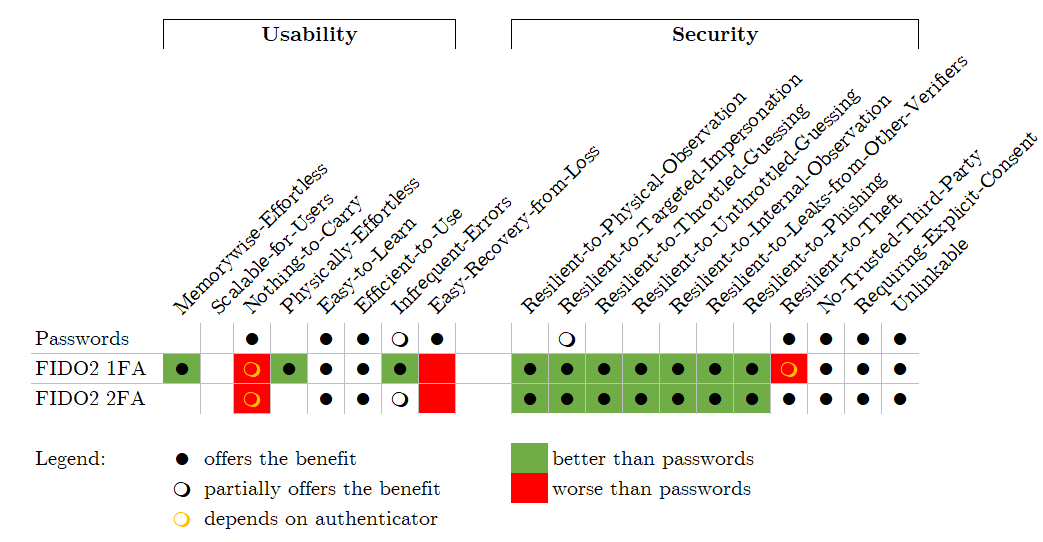
\includegraphics[width=1.8\columnwidth]{Figures/bonneau_matrix.png}
    \caption[Comparison of Authentication Methods]{Comparison of standard passwords with FIDO 1FA/2FA using a modified version of the framework proposed by Bonneau et al (2012)}
    \label{fig:bonneau_matrix}
\end{figure*}

\noindent The security perspective is also pretty straightforward: As nothing is entered by the user (except maybe a PIN), \ac{fido2} is resilient to observation. The use of asymmetric cryptography for the assertions also protects sufficiently against all forms of guessing, internal observation (like keyloggers), leaks and phishing. Theft might be a problem depending on the authenticator used, especially if no second factor (PIN or fingerprint) is used on the security key itself.\\

\noindent As figure \ref{fig:bonneau_matrix} shows, both \ac{fido2} modes score exceptionally well. In fact, as is also mentioned in \cite{lyastani2020}, no other authentication method offers as many benefits as the former.